\documentclass[]{article}
\usepackage[margin=1.1in, portrait]{geometry}
\usepackage{amsmath}
\usepackage{amssymb}
\usepackage{amsthm}
\usepackage{mathrsfs}
\usepackage[english]{babel}
\usepackage{multirow}
\usepackage{graphicx}
\newtheorem{stel}{Stelling}
\usepackage{float}
\usepackage{textcomp}
\usepackage{footmisc}
\usepackage[colorlinks=true, urlcolor=blue, linkcolor=blue, citecolor=blue, pdfborder={0 0 0}, linktoc=page]{hyperref}
\setlength{\parindent}{0 pt}
\usepackage{etoolbox}
\usepackage{scrextend}

\newcommand{\ba}{\begin{addmargin}[9mm]{0cm}}
\newcommand{\ea}{\end{addmargin}}
\newcommand{\cm}{\color{blue} \hspace{3mm}}


\title{\vspace{0cm} \huge \textsc{3D-RT: 3D Radiative Transfer} \\
                \vskip3mm \textsc{ Background Physics} }

\author{\large Frederik De Ceuster}
\date{}


\begin{document}

\maketitle

\vskip5cm

\begin{abstract}
This report aims to explain some of the physics behind the calculations done in the 3D-RT code.
\end{abstract}

\vskip5cm

\tableofcontents

\newpage


\section{General}

3D-RT is a multipurpose accelerated 3D radiative transfer code. Given a gas with a density and velocity distribution, an external radiation field and a provisional chemical composition, it selfconsistently calculates the temperature, level populations and chemical composition of the gas. 3D-RT is a ray-tracing code, meaning that to solve for the transport of electromagnetic radiation, the radiative transfer equation is solved along a set of rays.

\bigskip

The first version of 3D-RT is mainly based on 3D-PDR \cite{3DPDR}. The main difference is that in 3D-RT the radiative transfer is solved exactly and not in the Sobolev or large velocity gradient (LVG) approximation.

\bigskip

The code is mainly written in C with some features of C++. For the ray tracing the discretization scheme of the unit sphere is used from HEALPix\footnote{\url{https://healpix.jpl.nasa.gov}}. The chemical rate equations are solved using the CVODE solver provided in SUNDIALS\footnote{\url{https://computation.llnl.gov/projects/sundials}}. Most of the linear algebra is done using the Eigen\footnote{\url{http://eigen.tuxfamily.org}} library.



\section{Chemistry}


\section{Radiative transfer}

The \emph{intensity} $I_{\nu}\equiv I( \textbf{x},t;\hat{\textbf{n}},\nu)$ is defined as the energy $d\mathcal{E}$ propagated through a surface $d^{2}\textbf{S}$, in the direction $\hat{\textbf{n}}$, over a solid angle $d^{2}\omega$, within the frequency bin $[\nu,\nu+d\nu]$, in a time $dt$.
\begin{equation}
	d\mathcal{E} = I_{\nu} \ \ \hat{\textbf{n}} \cdot d^{2}\textbf{S} \ d^{2}\omega \ d\nu \ dt
\end{equation}
For simplicity we only consider the time-independent problem. (Add figure.)

\bigskip

The \emph{radiative transfer equation} expresses how much the intensity of the electromagnetic radiation in a certain frequency bin at a certain point changes in a certain direction.
\begin{equation}
\hat{\textbf{n}} \cdot \nabla I_{\nu}(\textbf{x},\hat{\textbf{n}}) \ = \ \eta_{\nu}(\textbf{x},\hat{\textbf{n}}) - \chi_{\nu}(\textbf{x}) I_{\nu}(\textbf{x},\hat{\textbf{n}})
\end{equation}
One can see that in this equation $\eta_{\nu}(\textbf{x},\hat{\textbf{n}})$ is the \emph{emissivity} which adds to the intensity and $\chi_{\nu}(\textbf{x})$ is the \emph{opacity} of the medium, which attenuates the intensity. Note that we assumed that the opacity is independent of the direction in which we look.


\subsection{Feautrier solution method}

To solve the radiative transfer equation along a ray we use the Feautrier method. The basic idea of the Feautrier method is to write the transfer equation as a second order instead of first order differential equation. Let us first make a distinction between the radiation travelling up and down a ray. Define
\begin{equation}
\begin{cases}
\ I^{+}_{\nu}(\textbf{x},\hat{\textbf{n}})  &\equiv \ I_{\nu}(\textbf{x},\hat{\textbf{n}}) \\
\ I^{-}_{\nu}(\textbf{x},\hat{\textbf{n}})  &\equiv \ I_{\nu}(\textbf{x},-\hat{\textbf{n}}) .
\end{cases}
\end{equation}
Using these definitions we can introduce the new variables
\begin{equation}
\begin{cases}
\ u_{\nu}(\textbf{x},\hat{\textbf{n}})  &\equiv \ \frac{1}{2}\big( I^{+}_{\nu}(\textbf{x},\hat{\textbf{n}}) + I^{-}_{\nu}(\textbf{x},\hat{\textbf{n}}) \big) \\
\ v_{\nu}(\textbf{x},\hat{\textbf{n}})  &\equiv \ \frac{1}{2}\big( I^{+}_{\nu}(\textbf{x},\hat{\textbf{n}}) - I^{-}_{\nu}(\textbf{x},\hat{\textbf{n}}) \big) .
\end{cases}
\end{equation}
The transfer equation for each of these new variables reads
\begin{equation}
\begin{cases}
\ \hat{\textbf{n}} \cdot \nabla u_{\nu}(\textbf{x},\hat{\textbf{n}}) &= \ \frac{1}{2} \big( \eta_{\nu}(\textbf{x},\hat{\textbf{n}}) + \eta_{\nu}(\textbf{x},-\hat{\textbf{n}}) \big) - \chi_{\nu}(\textbf{x}) u_{\nu}(\textbf{x},\hat{\textbf{n}}) \\
\ \hat{\textbf{n}} \cdot \nabla v_{\nu}(\textbf{x},\hat{\textbf{n}}) &= \ \frac{1}{2} \big( \eta_{\nu}(\textbf{x},\hat{\textbf{n}}) - \eta_{\nu}(\textbf{x},-\hat{\textbf{n}}) \big) - \chi_{\nu}(\textbf{x}) v_{\nu}(\textbf{x},\hat{\textbf{n}}) .
\end{cases}
\end{equation}
For a certain ray in direction $\hat{\textbf{n}}$ we can define the derivative along that ray and the optical depth as
\begin{equation}
\frac{d}{ds} \ \equiv \ \hat{\textbf{n}} \cdot \nabla \hspace{1cm} \text{and} \hspace{1cm} d\tau_{\nu} \ \equiv \ \chi_{\nu}(\textbf{x}) ds.
\end{equation}
By adding and subtracting the two forms of the transfer equation and substituting the results we find
\begin{equation}
\frac{d^{2} u_{\nu}(\textbf{x},\hat{\textbf{n}})}{d \tau_{\nu}^{2}} \ = \ u_{\nu}(\textbf{x},\hat{\textbf{n}}) - \frac{1}{2}\big( S_{\nu}(\textbf{x},\hat{\textbf{n}}) + S_{\nu}(\textbf{x},-\hat{\textbf{n}}) \big) + \frac{1}{2} \frac{d}{d\tau_{\nu}} \big( S_{\nu}(\textbf{x},\hat{\textbf{n}}) -  S_{\nu}(\textbf{x},-\hat{\textbf{n}}) \big) ,
\label{Feau}
\end{equation}
where the source function is defined as usual. Note that this is not the usual Feautrier equation since we did not assume that the emissivity is isotropic. This is neded if we want to consider scattering.

\bigskip

Now the problem is solved by discretizing $\tau_{\nu}$ and solve equation (\ref{Feau}) numerically. For simplicity, let us first consider the monochromatic an isotropic case. The straightforward generalization can be found in \cite{Mihalas_s, MihalasMihalas}. Consider the discretized grid as shown in figure \ref{grid}.
\begin{figure}[H]
	\centering
	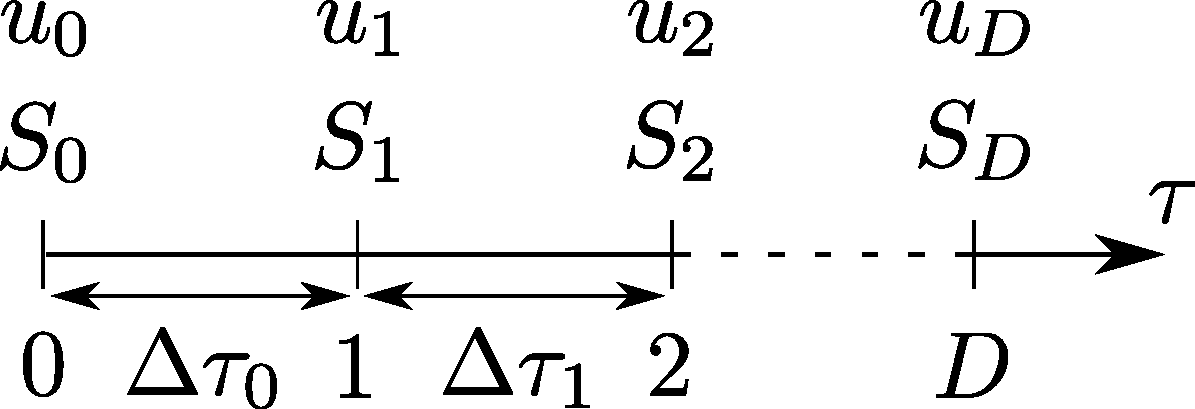
\includegraphics[scale=.5]{Images/grid.pdf}
	\caption{Discretization along the optical depth $\tau$.}
	\label{grid}
\end{figure}


Given the above discretization, the discretized version of (\ref{Feau}) then reads
\begin{equation}
\frac{\dfrac{u_{d+\frac{3}{2}}-u_{d+\frac{1}{2}}}{\Delta\tau_{d+1}}-\dfrac{u_{d+\frac{1}{2}}-u_{d-\frac{1}{2}}}{\Delta\tau_{d}}}{\Delta\tau_{d+\frac{1}{2}}} = - S_{d+\frac{1}{2}} + u_{d+\frac{1}{2}} ,
\label{dis}
\end{equation}
where we used
\begin{equation}
\begin{split}
\Delta\tau_{d} &\equiv \tau_{d+\frac{1}{2}} - \tau_{d-\frac{1}{2}} , \\
\Delta\tau_{d+\frac{1}{2}} &\equiv \frac{1}{2}\big(  \tau_{d+1} + \tau_{d}\big) .
\end{split}
\end{equation}
The discretized equation (\ref{dis}) can be rewritten as
\begin{equation}
-A_{d} \ u_{d-\frac{1}{2}} + B_{d} \ u_{d+\frac{1}{2}}  -C_{d} \ u_{d+\frac{3}{2}} \ = \ S_{d+\frac{1}{2}},
\label{rec}
\end{equation}
where we defined
\begin{equation}
\begin{split}
A_{d} &\equiv \frac{1}{\Delta\tau_{d} \ \Delta\tau_{d+\frac{1}{2}}} , \\
B_{d} &\equiv 1  + A_{d} + C_{d} , \\
C_{d} &\equiv \frac{1}{\Delta\tau_{d+1} \ \Delta\tau_{d+\frac{1}{2}}} .
\end{split}
\end{equation}
This enables us to write the descretized transfer equation in matrix form
\begin{equation}
\left( \begin{matrix}
B_{1} & -C_{1} & 0 & \cdots & 0 \\
-A_{2} & B_{2} & -C_{2} & \cdots & 0 \\
0 & -A_{3} & B_{3} & \cdots & 0 \\
\vdots & \vdots & \vdots & \ddots & \vdots \\
0 & 0 & 0 & \cdots & B_{D}
\end{matrix}\right)
\left( \begin{matrix}
u_{\frac{1}{2}} \\ u_{\frac{3}{2}} \\ u_{\frac{5}{2}} \\ \vdots \\ u_{D-\frac{1}{2}}
\end{matrix}\right)  = \left( \begin{matrix}
S_{\frac{1}{2}} \\ S_{\frac{3}{2}} \\ S_{\frac{5}{2}} \\ \vdots \\ S_{D-\frac{1}{2}}
\end{matrix}\right)
\end{equation}
One can solve this tridiagonal matrix equation be elimination and back-substitution. One can relate the first element to the second. From the first line one can find
\begin{equation}
u_{\frac{1}{2}} = S_{\frac{1}{2}} / B_{1} + C_{1}/B_{1} \ u_{\frac{3}{2}} .
\end{equation}
Now one can show that it is always possible to write $u_{d+\frac{1}{2}}$ in terms of $u_{d+\frac{3}{2}}$ as
\begin{equation}
u_{d+\frac{1}{2}} = v_{d} + D_{d} \ u_{d+\frac{3}{2}}  .
\end{equation}
Substituting this in (\ref{rec}) we can write
\begin{equation}
u_{d+\frac{1}{2}} = \left( B_{d} - A_{d} D_{d-1} \right)^{-1} \left( S_{d+\frac{1}{2}} + A_{d} \ v_{d-1} \right)   + \left( B_{d} - A_{d} D_{d-1} \right)^{-1} C_{d}  \ u_{d+\frac{3}{2}}  ,
\label{rec2}
\end{equation}
from this we can simply read the two coefficients
\begin{equation}
\begin{split}
v_{d} &= \left( B_{d} - A_{d} D_{d-1} \right)^{-1} \left( S_{d+\frac{1}{2}} + A_{d} \ v_{d-1} \right), \\
D_{d} &= \left( B_{d} - A_{d} D_{d-1} \right)^{-1} C_{d} .
\end{split}
\end{equation}
Now it is clear that to find all $u_{d+\frac{1}{2}}$, we first need to calculate all $D_{d}$ and simultaneously we can calculate the $v_{d}$, to then substitute these in (\ref{rec2}) to find the $u_{d+\frac{1}{2}}$.


\subsection{Scattering}

So far we only considered an absorption term $\chi_{\nu}(\textbf{x})$ and an emission term $\eta_{\nu}(\textbf{x},\hat{\textbf{n}})$. However, there is a third important process by which electromagnetic radiation can interact with the medium: scattering. The radiation interacts with the medium such that it is deflected. We can see this process as an absorption of radiation in a certain direction followed by emission in another direction. Note that this is why we allowed the emissivity to depend on the direction in which we look. The transfer equation including the scattering can be written as follows
\begin{equation}
\hat{\textbf{n}} \cdot \nabla I_{\nu}(\textbf{x},\hat{\textbf{n}}) \ = \ \eta_{\nu}(\textbf{x},\hat{\textbf{n}}) \ + \ \chi_{\nu}^{\text{sca}}(\textbf{x}) \int \text{d} \hat{\textbf{n}}' \ \Phi(\hat{\textbf{n}},\hat{\textbf{n}}') I_{\nu}(\textbf{x},\hat{\textbf{n}}') \ - \ \big( \chi_{\nu}(\textbf{x}) + \chi_{\nu}^{\text{sca}}(\textbf{x}) \big) I_{\nu}(\textbf{x},\hat{\textbf{n}}).
\label{RTEscat}
\end{equation}
The opacity gets an extra contribution from the radiation that is scattered out of the direction under consideration and the emissivity gets a contribution from the radiation of every direction that is scattered into the direction under consideration, hence the integral. $\Phi(\hat{\textbf{n}},\hat{\textbf{n}}')$ is the scattering phase function. It gives the angular distribution of the scattered radiation, i.e. the probability for incoming radiation from direction $\hat{\textbf{n}}'$ to be scattered into direction $\hat{\textbf{n}}$.

\bigskip

Including scattering in the transfer equation makes it a lot harder to solve: we need to know the radiation coming from all directions in order to solve for the radiation in a certain direction. We can overcome this difficulty by solving the equation iteratively. Let us first write equation (\ref{RTEscat}) in semi-discrete form where we only discretize the rays.
\begin{equation}
\frac{d I_{\nu}(\textbf{x},r)}{ds} \ = \ \eta_{\nu}(\textbf{x},r) \ + \ \chi_{\nu}^{\text{sca}}(\textbf{x}) \ \sum_{r' \neq r} \Phi(r,r') I_{\nu}(\textbf{x},r') \ - \ \Big( \chi_{\nu}(\textbf{x}) + \big( 1 - \Phi(r,r) \big) \chi_{\nu}^{\text{sca}}(\textbf{x}) \Big) I_{\nu}(\textbf{x},r).
\label{RTEscat}
\end{equation}


\section{Thermal balance}


\subsection{Dust temperature}



\subsection{Heating}



\subsection{Cooling}

For the moment the only cooling mechanism that is implemented is radiative cooling.

\subsubsection{Radiative cooling}

A gas can (locally) cool by radiative cooling when radiation from a certain region can escape i.e. the radiation is emitted by a region but not absorbed in that same region. The emission can be either spontaneous or stimulated.

\bigskip

The rate of energy emission in a frequency bin $\nu_{ij}$ can be given by
\begin{equation}
\dot{\mathcal{E}} \ = \ \dot{\mathcal{E}}_{\text{spontaneous emission}} + \dot{\mathcal{E}}_{\text{stimulated emission}} - \dot{\mathcal{E}}_{\text{absorption}} .
\end{equation}
The last term is needed because the stimulated emission will be counter acted by absoption. Using the definitions of the Einstein coefficients we can rewrite this as
\begin{equation}
\dot{\mathcal{E}} \ = \ h\nu_{ij} \ \phi_{\nu} \Big( A_{ij} \ n_{i}  + J_{\nu} \left( B_{ij} \ n_{i} - B_{ji} \ n_{j} \right) \Big).
\end{equation}
In terms of the line source function $S_{ij}$ the result can be written slightly more compact
\begin{equation}
\dot{\mathcal{E}} \ = \ h\nu_{ij} \ A_{ij} \ n_{i}  \phi_{\nu} \left( 1  - \frac{J_{\nu}}{S_{ij}} \right).
\end{equation}
The total radiative cooling is giver by the expression above for every downward transition i.e.
\begin{equation}
\dot{\mathcal{E}} \ = \ \sum_{j} \sum_{i>j} h\nu_{ij} \ A_{ij} \ n_{i}  \phi_{\nu} \left( 1  - \frac{J_{\nu}}{S_{ij}} \right).
\end{equation}
This is the way in which the radiative cooling is implemented in the code (\texttt{cooling.cpp}).


\newpage

\bibliography{library}
\bibliographystyle{ieeetr}



\end{document}
